\cotefile{162-5}
\scanpage{35}
premier. Comme applic\deleted{t}ation, Quillen obtient une interprétation faisceauti-
que de la cohomologie d'un ensemble semi-simplicial à coéfficients dans un
systême \inserted{local} con\deleted{tra}variant \inserted{$F$} \deleted{\unsure{de|dx}}(défini classiquement par le complexe cosimplicial
\margin{$\prod$ ?} des $C^n(F) = \rlap{\begin{tikzpicture}[overlay,x=1em,y=1em,baseline=0pt]\draw[black!35,line width=.3pt,rotate=25] (.40,-.20) ellipse (1.15 and .85);\end{tikzpicture}}\coprod\limits_{x\in X_n} F(x)$): on considère le systême local contravariant
défini par $F$, on l'interprète comme un faisceau sur \inserted{$T(X)$ i.e. objet de} $(\mathrm{Ssimpl})_{/X}$, et on
prend sa cohomologie. - Cependant, quand $F$ est un systême de coéfficien\unsure{\deleted{s}t|\deleted{t}s}s
cov\deleted{\unsure{r}}ariant pas nécessairement local, on n'a tjrs pas d'interp\unsure{\deleted{é}r|\deleted{r}é}étation de se\unsure{\deleted{n}s|\deleted{s}n}
groupes de cohomologie classiques en t ermes faisc\deleted{d}eautiques; ni, lorsque $F$
est co\deleted{\unsure{v}}n\deleted{a}tr\deleted{i}a\deleted{a}v\deleted{\unsure{n}}a\deleted{t}r\deleted{\unsure{,}}iant, de son homologie, ou inversement de sa cohomologie
faisceautique en termes classiques.

A propos de la notion de foncteur qui est un homotopisme. Quillen
montre qu\deleted{e}'un tel foncteur $F:C\longrightarrow C'$ induit une équiva\unsure{\deleted{n}l|\deleted{l}n}ence entre la sous-
catégorie triangulée \inserted{$D^b_{lc}(C')$} de la catégorie \inserted{dérivée \inserted{bornée} de celle \deleted{des}} des faisceaux abéliens sur $C'$, dont
les faisceaux de cohomologie sont des systêmes locaux, et la catégorie ana-
logue pour $C$; \deleted{Il s'en} et réciproquement. \deleted{Pour la partie directe} On peut
dans cet énoncé introduire aussi n'importe quel anneau de base (à condition
de le supposer $\neq 0$ dans le cas de la réciproque); \deleted{constant} la partie directe
vaut aussi avec un anneau de boefficients pas néc. constant, mais constant
tordu. Je pense que ce résultat (facile) doit pouvoir se généraliser ainsi:
Soit $f:X\quad X'$ un morphisme de topos qui soit tel que pour tout \deleted{systême}
faisceau loc. const. sur $X'$, $f$ induise un isomorphisme sur les cohomologies
(avec cas non commutatif inclus). Supposons que \deleted{\unsure{le} (\unsure{topos} $X$) soit} \inserted{$X$ et $X'$} \uline{localement}
\margin{
\begin{tikzpicture}[x=1em,y=1em,baseline=-.1em]\draw[line width=.65pt] (0,0) ellipse (.12 and .13);\draw[line width=.85pt] (.08,.1) .. controls (.20,.44) and (.44,.84) .. (.52,.99);\end{tikzpicture}} \margin{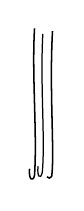
\begin{tikzpicture}[x=1em,y=1em]\draw[line width=.55pt] (0,5.5) .. controls (-.10,3.8) and (.10,1.7) .. (0,.20) .. controls (-.05,-.06) and (-.22,.02) .. (-.18,.43);\draw[line width=.45pt] (.30,5.3) .. controls (.20,3.5) and (.39,1.5) .. (.28,.29) .. controls (.21,.02) and (.08,.15) .. (.13,.52);\draw[line width=.55pt] (.65,5.4) .. controls (.53,3.3) and (.73,1.0) .. (.62,.15) .. controls (.58,.05) and (.49,.10) .. (.45,.14);\end{tikzpicture}} \uline{homotopiquement trivial}, i.e. que \deleted{tout} pour tout entier $n$\inserted{$\geq 1$}, tout objet $U$ \deleted{de}
\deleted{$X$}$'$ ait un \inserted{recouvrement} \deleted{revêtement} par des $U_i\longrightarrow U$, tels que a) tout systême local sur $U$
devient constant sur $U_i$, et toute section sur $U$ devient constante sur $U_i$,
et b) pour tout \deleted{systême} groupe abélien $G$, les $H^j(U,G)\unsure{\longrightarrow|\longleftrightarrow} H^j(U_i,G)$ sont
nuls pour $1\leq j\leq n$. Alors le foncteur $D^b_{lc}(X')\longrightarrow D^b_{lc}(X)$ induit par $f$ est

\figure{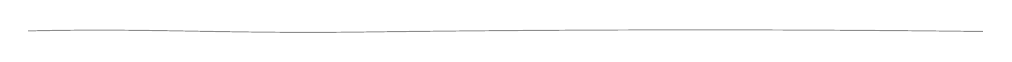
\begin{tikzpicture}[x=\linewidth,y=1em]\draw[black!45,line width=.35pt] (0,0) .. controls (.13,.10) and (.20,-.10) .. (.35,-.04) .. controls (.58,.06) and (.80,.06) .. (1,-.02);\end{tikzpicture}}

\margin{
\begin{tikzpicture}[x=1em,y=1em,baseline=-.1em]\draw[line width=.65pt] (0,0) ellipse (.12 and .13);\draw[line width=.85pt] (.08,.1) .. controls (.20,.44) and (.44,.84) .. (.52,.99);\end{tikzpicture} Attention, cette condition n'est typiquement \uline{pas} satisfaite par les schémas avec leur topologie étale (mais bien par \unsure{schémas} l. noeth. avec top. Zariski).}

\margin{34}
